\documentclass[tikz,border=8pt]{standalone}
\usepackage{amsmath,amssymb}
\usetikzlibrary{arrows.meta,calc,positioning}

% Generated by gen_hold.py from hold.stl -- edit the generator, not this file.
\begin{document}
\graphicspath{{figures/}{./}}
\begin{tikzpicture}[
    >={Stealth[length=4pt,width=3pt]},
    font=\sffamily\small,
    dim/.style={<->,thin,black!70},
    ext/.style={thin,black!35},
    lead/.style={thin,black!55},
    env/.style={acc,thick,dashed},
    hid/.style={steel,thin,densely dashed},
    ttl/.style={font=\sffamily\small\bfseries},
  ]
  \definecolor{wood}{RGB}{226,205,171}
  \definecolor{woodE}{RGB}{150,120,80}
  \definecolor{acc}{RGB}{0,102,170}
  \definecolor{hold}{RGB}{46,170,80}
  \definecolor{steel}{RGB}{95,105,118}

  % Real hold (hold.stl), drawn in mm. Bolt axis at Z = 0, bolts at X = +-15
  % (two pitches of the 15 mm grid), socket centre at Z = -14, 26 mm from the
  % wall, back plate 3 mm thick, depth 43 mm.
  \def\P{15}\def\R{30}\def\L{100}

  %% =============================== FRONT VIEW ===========================
  \begin{scope}[x=0.04cm,y=0.04cm]
    \fill[wood] (-50,-50) rectangle (50,50);
    \begin{scope}
      \clip (-50,-50) rectangle (50,50);
      \foreach \i in {-3,...,3}{\foreach \j in {-3,...,3}{
          \fill[woodE!85!black] ({\i*\P},{\j*\P}) circle (1.7);}}
    \end{scope}
    \node[anchor=south west,inner sep=0pt] at (-0.8064cm,-1.1622cm) {
\includegraphics[width=1.6167cm]{hold_front.png}};
    \foreach \hx in {-15,15}{
      \fill[steel] (\hx,0) circle (2.75);
      \fill[white] (\hx,0) circle (0.9);}
    \fill[acc] (0,-14) circle (1.0);
    \draw[env] (0,0) circle (\R);
    \fill[acc] (0,0) circle (0.8);

    \draw[ext] (-15,{0+4}) -- (-15,{0+22});  \draw[ext] (15,{0+4}) -- (15,{0+22});
    \draw[dim] (-15,{0+18}) -- (15,{0+18}) node[midway,fill=wood,inner sep=1pt] {$30$};
    \draw[ext] (17,0) -- (40,0);  \draw[ext] (2,-14) -- (40,-14);
    \draw[dim] (36,0) -- (36,-14) node[midway,fill=wood,inner sep=1pt,rotate=90] {$14$};
    \draw[lead] (0,-14) -- (-26,-38) node[below,font=\sffamily\footnotesize,fill=wood,inner sep=1pt] {socket centre};
    \draw[acc,thin,{Stealth[length=4pt,width=3pt]}-{Stealth[length=4pt,width=3pt]}]
          (0,0) -- (45:\R);
    \node[acc,font=\sffamily\footnotesize,fill=wood,inner sep=1pt] at (45:{\R+7}) {$R\,30$};

    \node[ttl,above=2mm] at (0,50) {Front view};
    \node[font=\sffamily\footnotesize,align=center,below=1.5mm] at (0,-50)
         {$2\times$ M3 bolts on grid holes\\ two pitches apart ($30$\,mm)};
  \end{scope}

  %% ==================== SIDE VIEW: section through the socket ===========
  \begin{scope}[shift={(3.3cm,0)},x=0.04cm,y=0.04cm]
    \fill[wood,draw=woodE] (-10,-50) rectangle (0,50);
    \foreach \j in {-3,...,3}{\fill[white] (-10,{\j*\P-1.7}) rectangle (0,{\j*\P+1.7});}
    \node[anchor=south west,inner sep=0pt] at (-0.0011cm,-1.1622cm) {
\includegraphics[width=1.7233cm]{hold_side.png}};
    % bolts are at X = +-15, hidden behind the side gusset: head on the plate, nut on the rear
    \begin{scope}[shift={(0,0)}]
      \draw[hid] (3,-2.75) rectangle (6,2.75);
      \draw[hid] (-12.5,-1.5) rectangle (3,1.5);
      \draw[hid] (-12.4,-2.75) rectangle (-10,2.75);
    \end{scope}
    \fill[acc] (26,-14) circle (1.0);

    \draw[env] (0,-\R) rectangle (\L,\R);
    \draw[ext] (0,-\R) -- (0,-52);  \draw[ext] (\L,-\R) -- (\L,-52);
    \draw[dim] (0,-48) -- (\L,-48) node[midway,fill=white,inner sep=1pt] {$100$};
    \draw[ext] (\L,\R) -- ({\L+18},\R); \draw[ext] (\L,-\R) -- ({\L+18},-\R);
    \draw[dim] ({\L+13},-\R) -- ({\L+13},\R)
          node[midway,fill=white,inner sep=1pt,rotate=90] {$\varnothing\,60$};
    \draw[ext] (43,{0+6}) -- (43,{0+26});
    \draw[dim] (0,{0+22}) -- (43,{0+22}) node[midway,fill=white,inner sep=1pt] {$43$};
    \draw[ext] (26,{-14-2}) -- (26,-42);
    \draw[dim] (0,-38) -- (26,-38) node[midway,fill=white,inner sep=1pt] {$26$};

    \node[ttl,above=2mm] at (45,50) {Side view};
    \node[font=\sffamily\footnotesize,align=center,below=1.5mm] at (45,-52)
         {seen along the wall; hidden bolts dashed,\\
          M3 nut on the rear face;\\ dot: socket centre (inside the bucket)};
  \end{scope}

  %% =============================== ISOMETRIC =============================
  % projection: x along the wall, z up, -y out of the wall toward the viewer
  \def\ax{0.0384}\def\ay{-0.0128}\def\bx{0.0256}\def\by{0.016}\def\cz{0.0416}
  \begin{scope}[shift={(12.4cm,0.3cm)},
                x={(\ax cm,\ay cm)},y={(\bx cm,\by cm)},z={(0cm,\cz cm)}]
    % A disc lying in the wall plane projects to a sheared ellipse spanned by the
    % x and z vectors; redefining y as z makes "circle" draw that ellipse.
    \begin{scope}[y={(0cm,\cz cm)}]
      \fill[wood,draw=woodE] (-52,-52) -- (52,-52) -- (52,37) -- (-52,37) -- cycle;
      \foreach \i in {-3,...,3}{\foreach \j in {-3,...,2}{
          \fill[woodE!85!black] ({\i*\P},{\j*\P}) circle (1.7);}}
    \end{scope}
    \draw[acc,thick] plot[domain=0:360,samples=73,smooth] ({\R*cos(\x)},0,{\R*sin(\x)});
    \node[anchor=south west,inner sep=0pt] at (-1.4491cm,-1.7916cm) {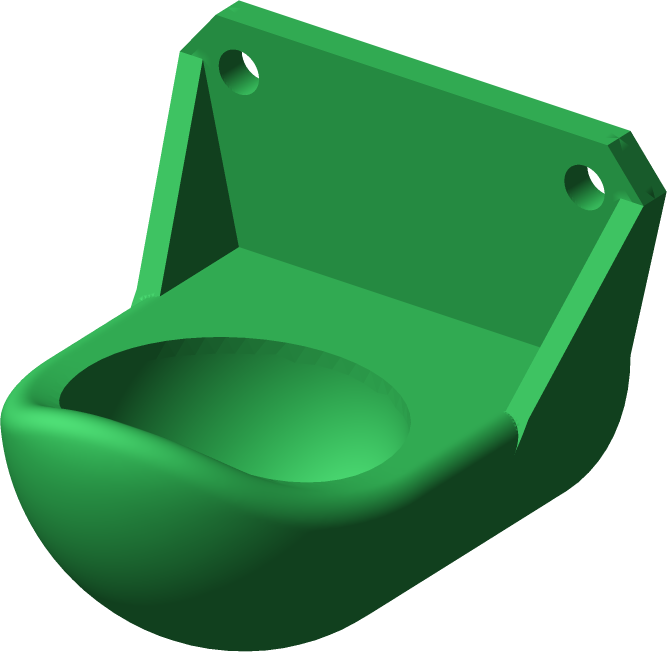
\includegraphics[width=2.2267cm]{hold_iso.png}};

    % envelope: silhouette generators at the tangent angle, front circle
    \pgfmathsetmacro{\ta}{atan(\cz*\bx/(\ay*\bx-\ax*\by))}
    \pgfmathsetmacro{\tb}{\ta+180}
    \fill[acc,opacity=0.08]
      plot[domain=\ta:\tb,samples=40,smooth] ({\R*cos(\x)},0,{\R*sin(\x)})
      -- plot[domain=\tb:\ta+360,samples=40,smooth] ({\R*cos(\x)},-\L,{\R*sin(\x)})
      -- cycle;
    \draw[acc,thick] ({\R*cos(\ta)},0,{\R*sin(\ta)}) -- ({\R*cos(\ta)},-\L,{\R*sin(\ta)});
    \draw[acc,thick] ({\R*cos(\tb)},0,{\R*sin(\tb)}) -- ({\R*cos(\tb)},-\L,{\R*sin(\tb)});
    \draw[acc,thick] plot[domain=0:360,samples=73,smooth] ({\R*cos(\x)},-\L,{\R*sin(\x)});
    \draw[acc,thin,densely dashed] (0,0,0) -- (0,{-\L-18},0);
  \end{scope}
  \node[ttl,anchor=south] at (12.4cm,2.75cm) {Envelope};
  \node[font=\sffamily\footnotesize,align=center,anchor=north] at (12.4cm,-2.85cm)
       {cylinder $\varnothing=60$\,mm, $L=100$\,mm,\\ axis normal to the wall,
        centred between the bolts};
\end{tikzpicture}
\end{document}
